\chapter{Исследовательская часть}

В данном разделе будет приведен пример работы реализации программы, проведен сравнительный анализ реализаций алгоритмов 
при различных ситуациях на основе полученных данных.

\section{Технические характеристики}

Технические характеристики устройства, на котором выполнялись замеры по времени, представлены далее:

\begin{itemize}
	\item процессор -- 2 ГЦ 4‑ядерный процессор Intel Core i5;
	\item оперативная память -- 16 ГБайт;
	\item операционная система -- macOS Venura 13.5.2. 
\end{itemize}

\section{Пример работы реализации программы}

В листинге \ref{lst:exmpl} приведен пример работы реализации программы.

\begin{lstlisting}[label=lst:exmpl,caption=Демонстрация работы реализации программы]
    ivanmamvriyskiy@MacBook-Pro-Ivan-2 main % python3 main.py
    Введите строку: Все будет хорошо!
    Введите подстроку: плохо
    Подстрока не найдена
    Подстрока не найдена

    ivanmamvriyskiy@MacBook-Pro-Ivan-2 main % python3 main.py
    Введите строку: Все будет хорошо!
    Введите подстроку: хорошо
    Стандартный алгоритм. Подстрока найдена на позиции 10
    Алгоритм Бойера-Мура. Подстрока найдена на позиции 10
\end{lstlisting}

\section{Цель исследования}
Целью исследования является проведение измерений количества сравнений и времени работы реализаций алгоритмов, необходимых для 
решения задачи поиска первого вхождения подстроки в строку в лучшем и худшем случае. 
На основе полученных оценок следует обосновать, какой из двух случаев представляет собой худший 
вариант: сценарий отсутствия подстроки длиной S или сценарий нахождения её в строке на последних S позициях.

\section{Ход исследования}
Исследование было проведено для двух различных сценариев расположения образца в строке: 
когда образец находился в конце строки и когда его не было в строке вообще. 
Замеры времени производились для строк разных размеров: 512, 1024, 2048, 4096 и 8192. 
Строка состояла из одинаковых элементов русского алфавита. 
В ходе замеров измерялись время выполнения реализаций алгоритмов и количество сравнений.

\section{Результаты исследования}

На рисунках \ref{img:endT} -- \ref{img:noT} представлены столбчатые диаграммы результатов замера времени для стандартного алгоритма и 
алгоритма Бойера-Мура. Замеры времени производятся в микросекундах. Также на рисунках \ref{img:endC} -- \ref{img:noC} представлены столбчатые диаграммы результатов замера 
количества сравнений.
\clearpage
\begin{figure}[h]
    \centering
    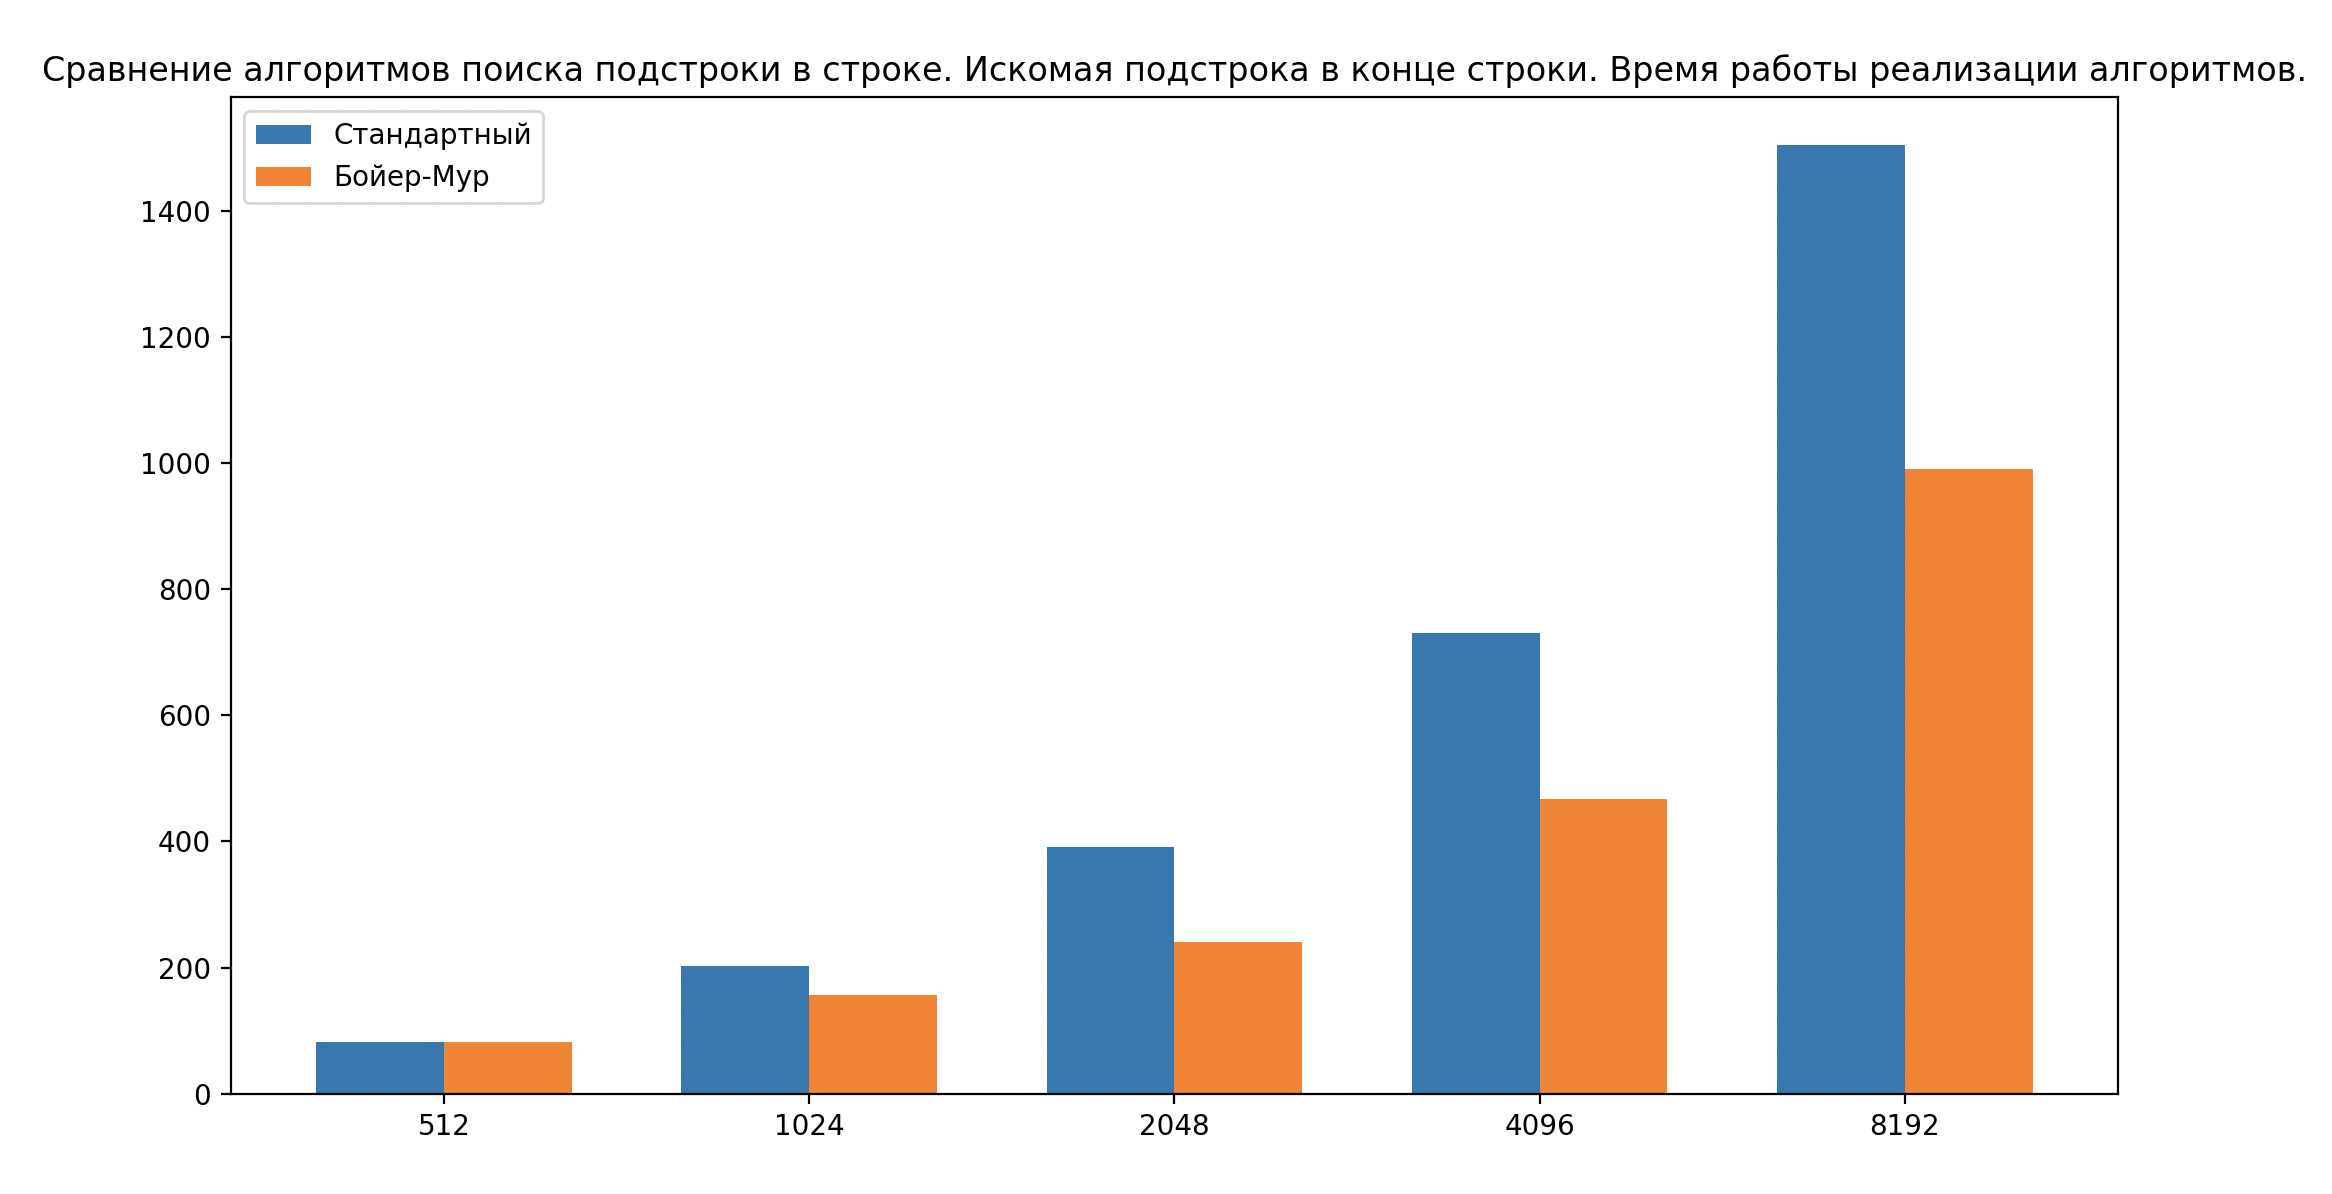
\includegraphics[width=1\linewidth]{img/endT.png}
    \caption{Результаты замера времени реализаций алгоритмов в случае, когда искомая подстрока находится в конце строки}
    \label{img:endT}
\end{figure}

\begin{figure}[h]
    \centering
    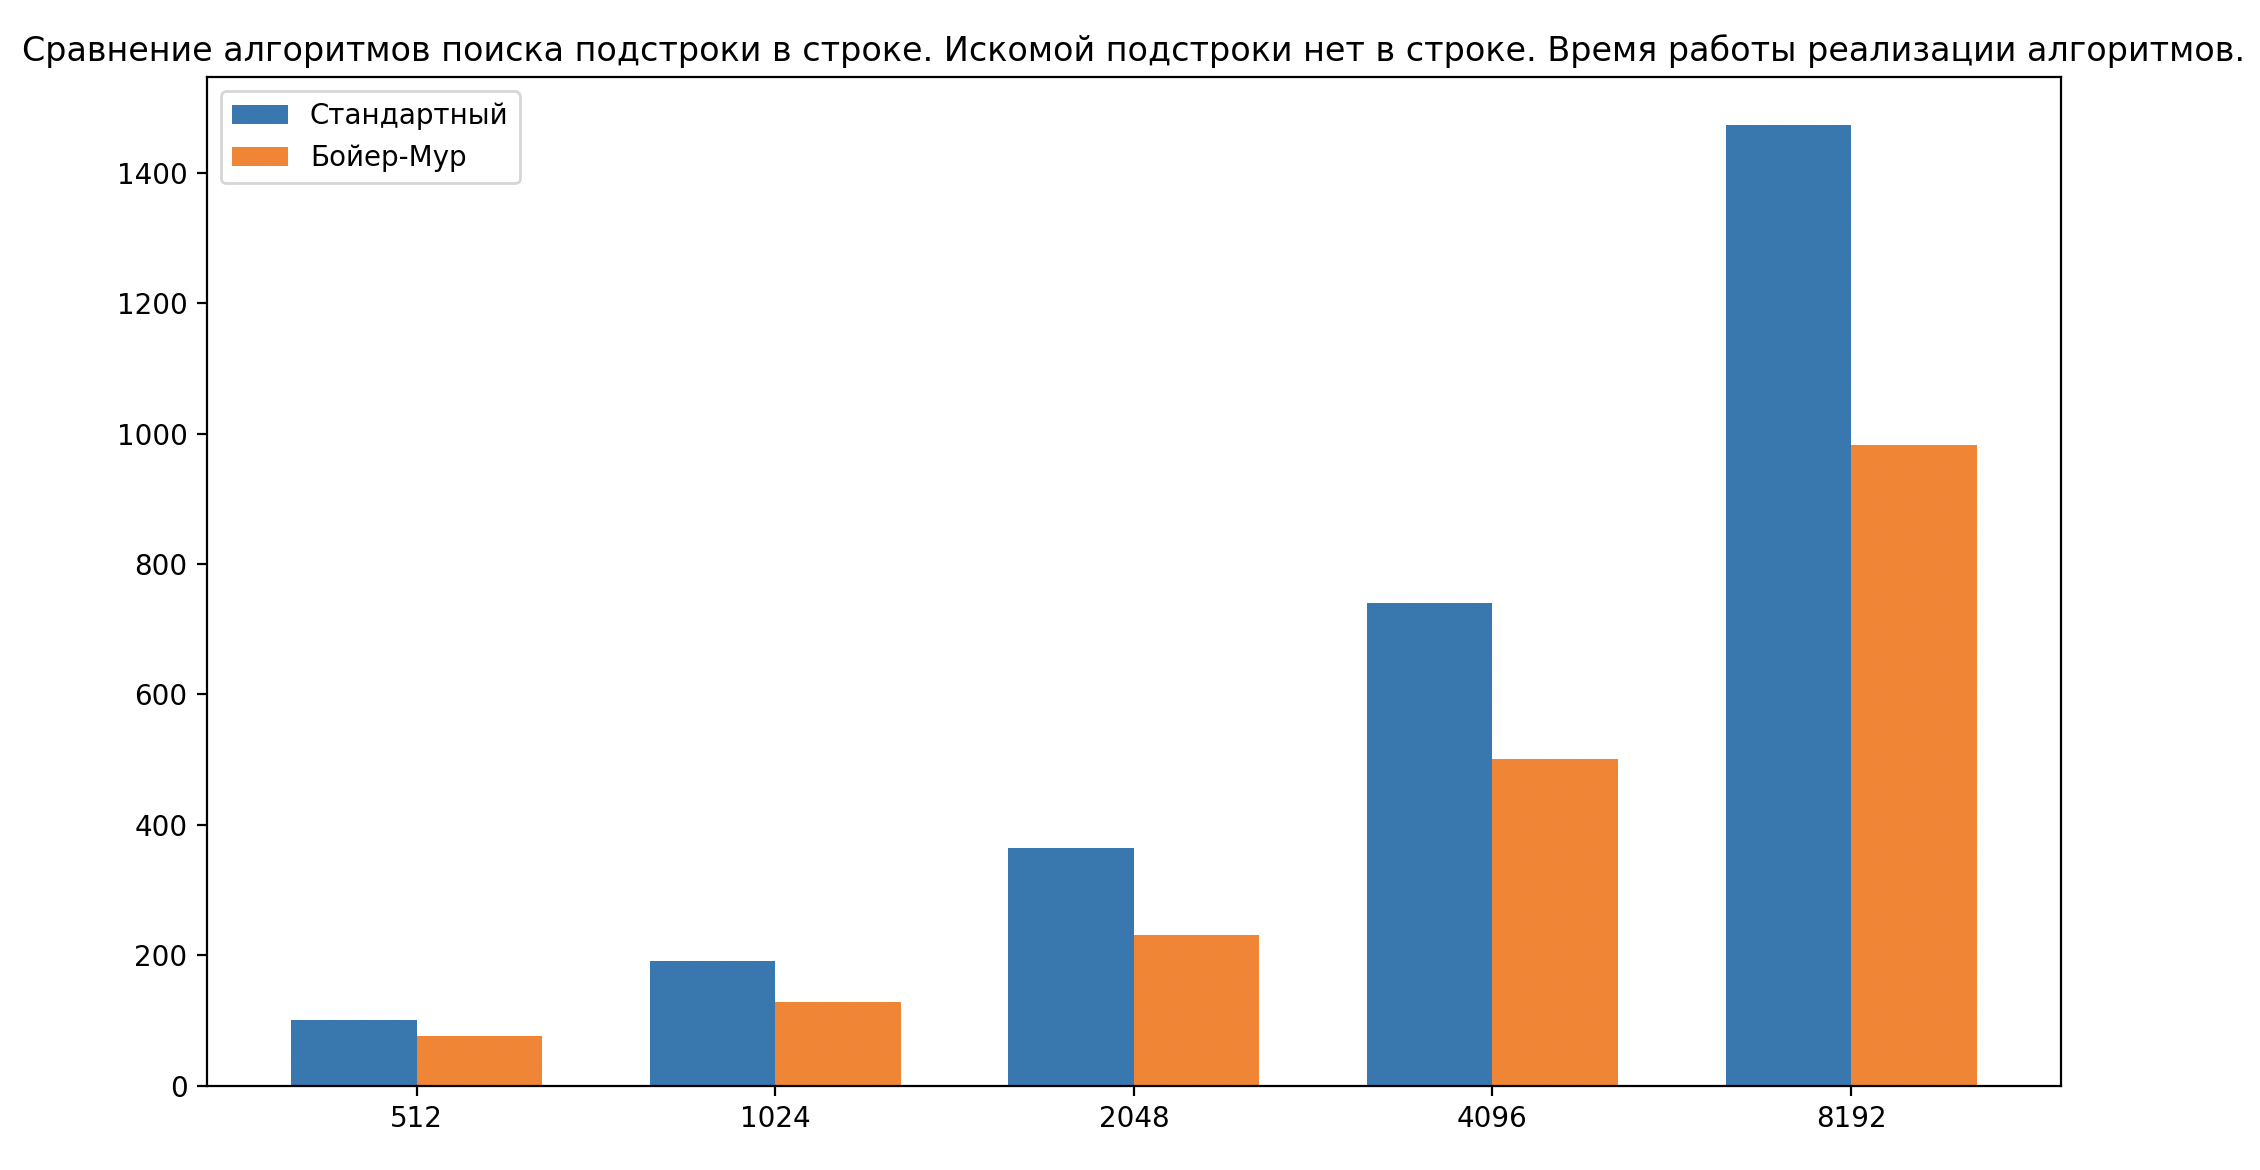
\includegraphics[width=1\linewidth]{img/noT.png}
    \caption{Результаты замера времени реализаций алгоритмов в случае, когда искомой подстроки нет в строке}
    \label{img:noT}
\end{figure}

\begin{figure}[h]
    \centering
    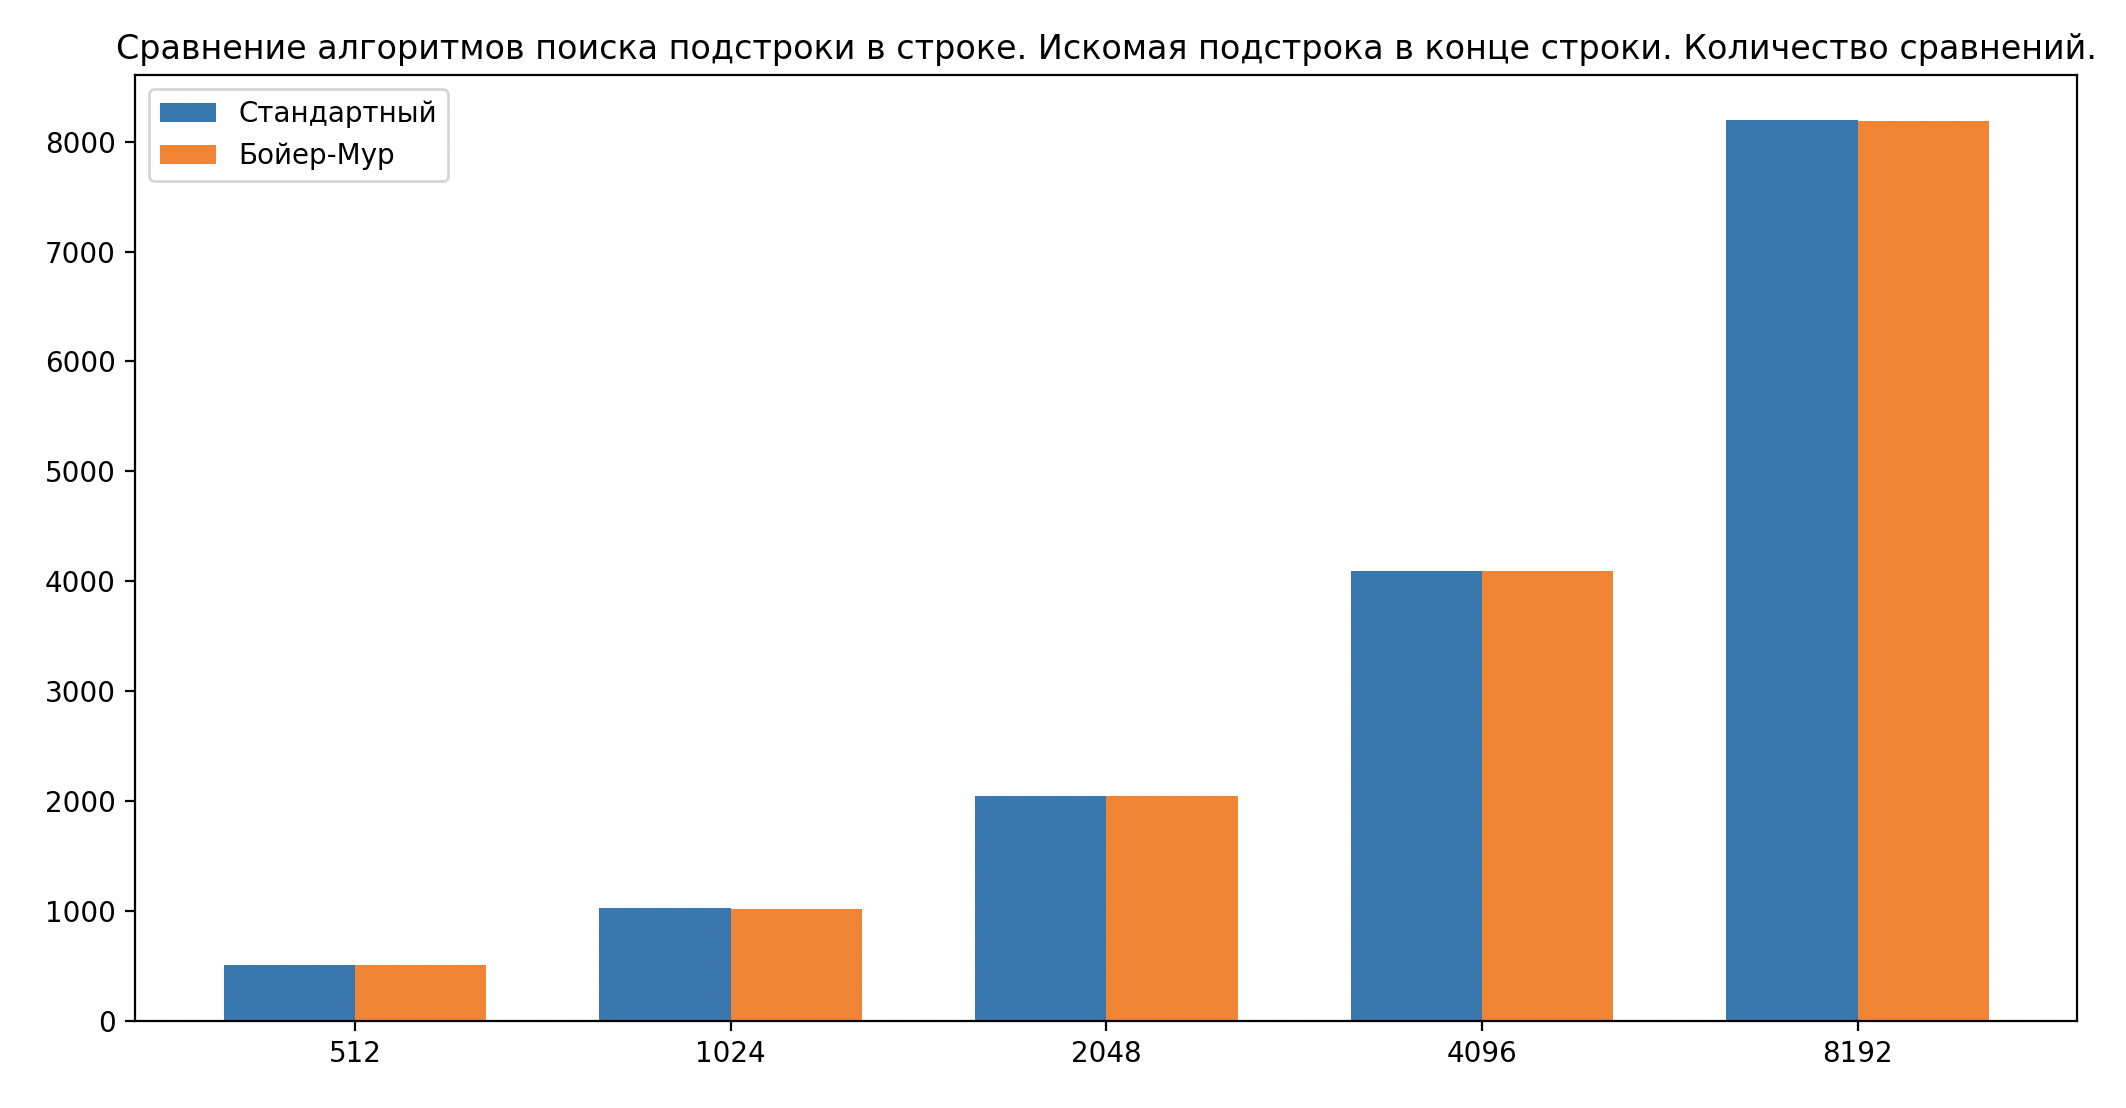
\includegraphics[width=1\linewidth]{img/endC.png}
    \caption{Результаты замера количества сравнений в случае, когда искомая подстрока находится в конце строки}
    \label{img:endC}
\end{figure}

\begin{figure}[h]
    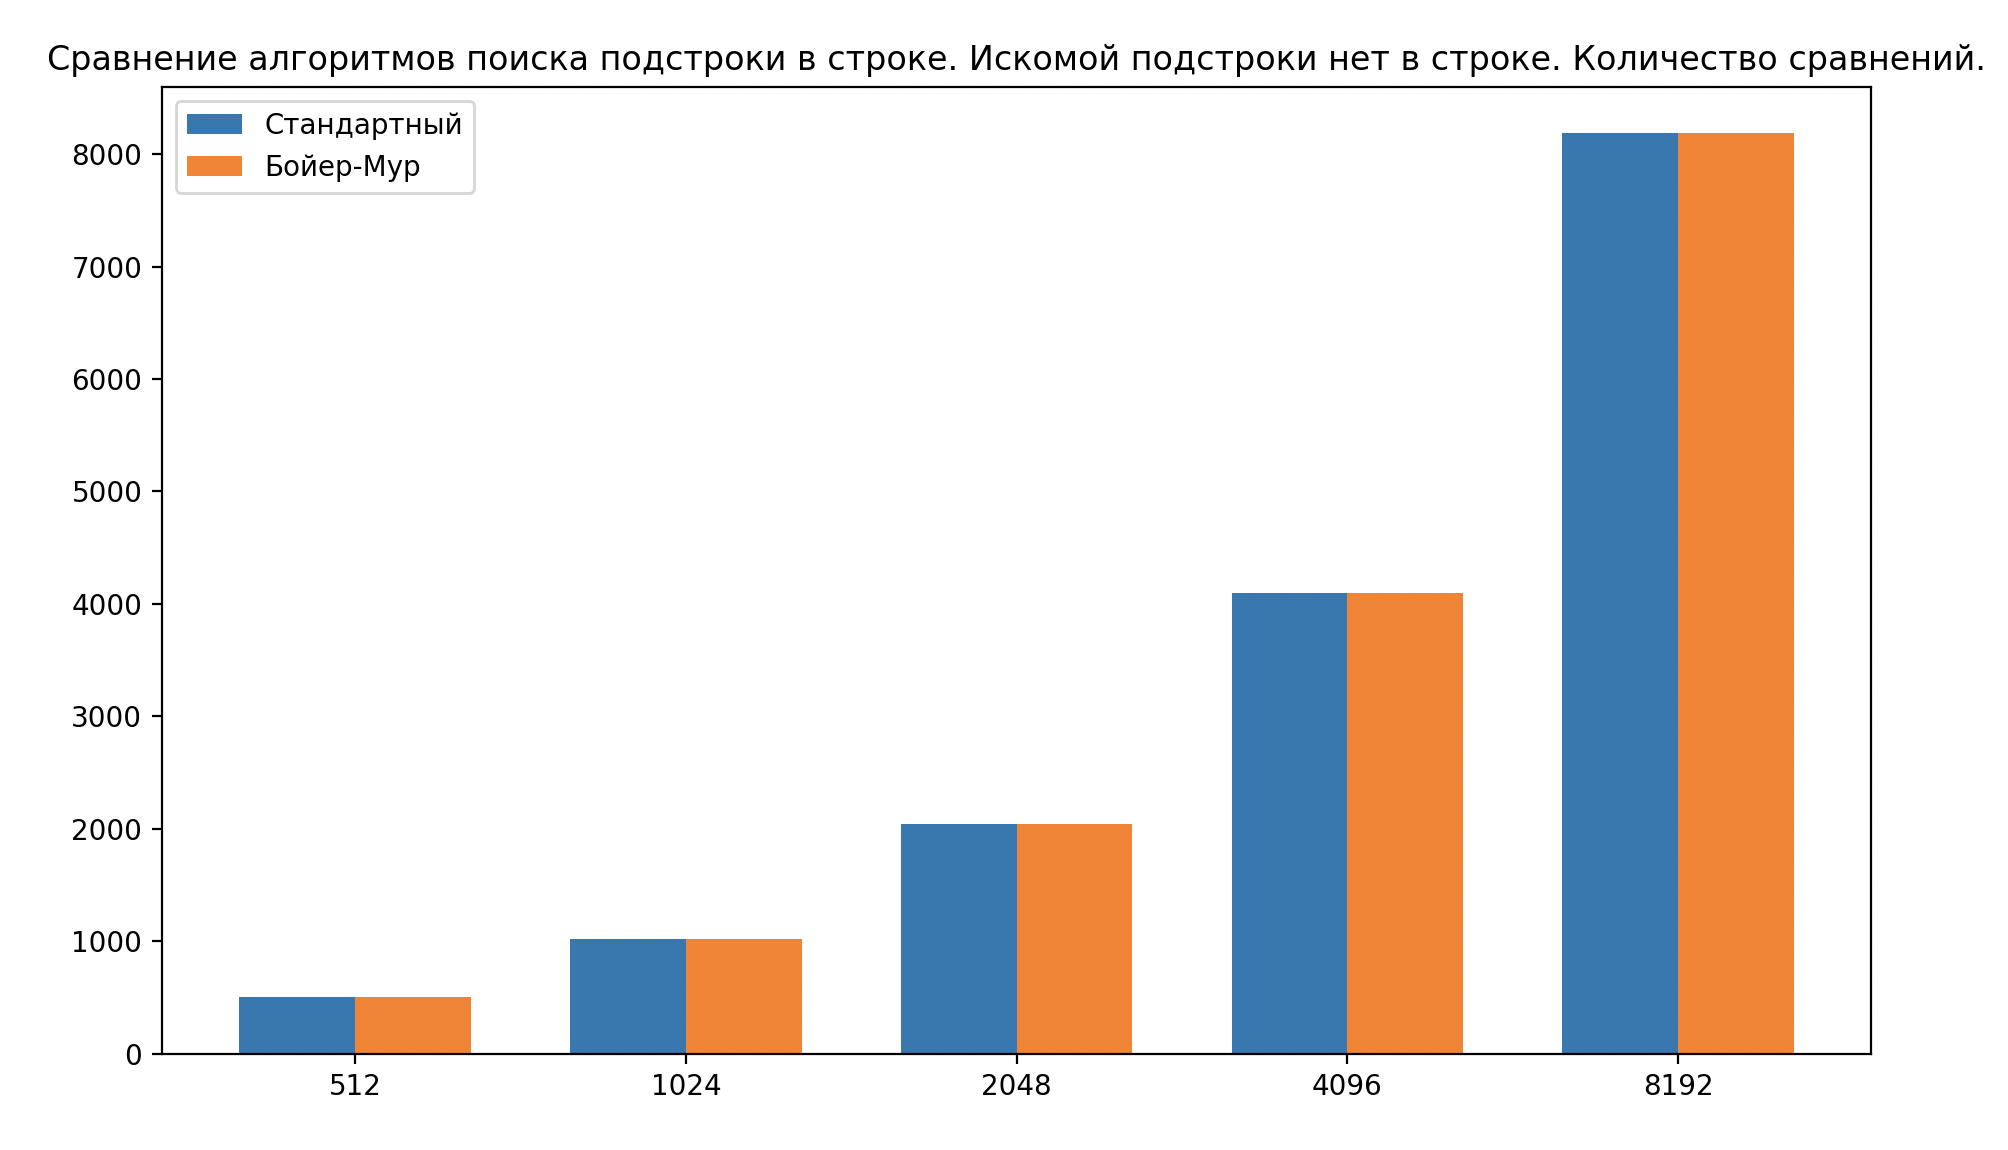
\includegraphics[width=1\linewidth]{img/noC.png}
    \caption{Результаты замера количества сравнений в случае, когда искомой подстроки нет в строке}
    \label{img:noC}
\end{figure}
\clearpage

По данным замерам можно сделать следующие выводы:
\begin{itemize}
    \item худшим случаем по времени выполнения как для реализации стандартного алгоритма, так и для реализации алгоритма Бойера-Мура
    является случай, когда подстроки нет в строке;
    \item худшим случаем по количеству сравнений для реализации стандартного алгоритма является
    случай, когда образец находится в конце строки, а для реализации алгоритма Бойера-Мура худшим
    является случай, когда подстроки нет в строке.
\end{itemize}


\section{Вывод}
Таким образом, наихудшим сценарием по количеству сравнений для реализации
стандартного алгоритма является тот, в котором подстрока расположена 
в конце строки, а наихудшим с точки зрения времени –- тот, где 
подстрока отсутствует в строке. В случае реализации алгоритма Бойера-Мура 
наихудшим сценарием как по количеству сравнений, так и по 
временным затратам является ситуация, когда подстрока отсутствует
в строке.

